\documentclass[conference]{IEEEtran}
% If the IEEEtran.cls has not been installed into the LaTeX system files,
% manually specify the path to it: e.g.,
% \documentclass[conference]{../sty/IEEEtran}

\usepackage[latin1]{inputenc}
\usepackage{graphicx,color,longtable,multirow,times,amsmath,url}
\usepackage[dvips]{epsfig}
\usepackage{textcomp}
\usepackage{verbatim}
\usepackage{algorithm}
\usepackage{algorithmic}
% correct bad hyphenation here
\hyphenation{}

\IEEEoverridecommandlockouts    % to create the author's affliation portion
                % using \thanks

\textwidth 178mm    % <------ These are the adjustments we made 10/18/2005
\textheight 239mm   % You may or may not need to adjust these numbes again
\oddsidemargin -7mm
\evensidemargin -7mm
\topmargin -6mm
\columnsep 5mm

\setlength{\textfloatsep}{8pt plus 2pt minus 2pt}
\setlength{\intextsep}{8pt plus 2pt minus 2pt}

\begin{document}


% paper title: Must keep \ \\ \LARGE\bf in it to leave enough margin.
\title{\ \\ \LARGE\bf Fighting to Survive: Evolving RTS Bots without Explicit Evaluation}

\author{A.J. Fern�ndez-Ares, P. Garc�a-S�nchez, A.M. Mora, P. A. Castillo and J.J. Merelo \thanks{Department of Architecture and Computer Technology, University of Granada, Spain, {\tt \{antares,pablogarcia\}@ugr.es, \{amorag,pedro,jmerelo\}@geneura.ugr.es}}}
% avoiding spaces at the end of the author lines is not a problem with
% conference papers because we don't use \thanks or \IEEEmembership
% use only for invited papers
%\specialpapernotice{(Invited Paper)}

% make the title area
\maketitle

\begin{abstract}
This paper proposes an evolutionary algorithm for evolving game bots that eschews a explicit fitness function for a fight between individuals implemented as a selection mechanism. Instead of measuring fitness by making the bots
perform certain tasks or fight against baseline bots, they fight with
each other and  on the winners  survive, passing  to the next
generation. Explicit evaluation is thus omitted and substituted by
explicit comparisons between bots. This algorithm has been designed as
an optimization method for the parameters of the behavioural engine of
bots for the RTS game Planet Wars, and has  two
objectives: first, to  deal better with the noisy nature of the fitness
function (the evaluation for the same individual may vary from one
time to another, due to the stochastic component of the combats); and
second, to obtain more general bots than those evolved considering a
specific opponent, which are optimized to fight against it, and so,
they are specialized bots. In addition, avoiding the evaluation step
ideally will reduce the algorithm time consumption.
% Todas estas cosas tienes que probarlas.
Three different approaches are proposed and compared, namely steady-state and generational implementations, and a pool-based approach in which a combat arena with potential individuals is considered. Each of them applies 1 vs
1 bots combats. 
*** RESULTS show that...***

%They implement different exploration versus
%exploitation tradeoffs in order to decide the best balance between
%these factors.  
% �Por qu� consideras todas estas cosas? �Por qu� es
% importante la exploraci�n frente a la explotaci�n en
% este tipo de trabajos?
% Antonio - porque pienso que es importante en todos los algoritmos de optimizaci�n decidir el justo equilibrio entre exploraci�n y explotaci�n. Pero no queda muy adecuado aqu�, as�q ue lo quito.
\end{abstract}


%
%%%%%%%%%%%%%%%%%%%%%%%%%%%%%%%   INTRODUCTION   %%%%%%%%%%%%%%%%%%%%%%%%%%%%%%%
%
\section{Introduction}
\label{sec:intro}
%
Evolutionary Algorithms (EAs) have been widely applied in a number of problems, including videogames \cite{Ponsen_EvLearn_RTS,co-evol-rts2006,Su-EAs_StrategySel09,cooperativebots_CIG2010,Cook_Platforming2012}. This metaheuristic performs very well in most of cases, but the presence
 of the so-called $noise$ in the evaluation process can make them do
 not work properly \cite{Genebot_JCST}. 

% citas sobre el tema, incluyendo los tuyso
                    % propios - JJ
This problem is quite common in the videogames scope, due to the
pseudo-stochasticity present in some factors, such as the game rules
or status the opponents' behaviour or the random initial condition,
which obviously have an influence on the score obtained by the bot,
which is usually the base (sometimes the only one) for giving a bot a
fitness in an evolutionary algorithm. 
This problem also arises when the opponents follow non-deterministic
Artificial Intelligence (AI) behavioural models, i.e. when they are
Non-Playing Characters (NPC) or $bots$, since their behaviour
considers stochastic factors which can influence the result of the
game, and can vary from time to time. % citas para todo.

Planet Wars, the RTS used in the Google AI Challenge
2010\footnote{http://planetwars.aichallenge.org/} is not an exception
when an EA is applied to improve bots for playing it
\cite{Genebot-IWANN2011,Genebot_CEC11,Genebot_CIG2012},  presenting
this problem in the fitness calculation \cite{Genebot_JCST}. The usual
solution consist in performing several evaluations for the same
individual (maybe in different maps or against different opponents)
and then compute its fitness value as an average or sum of all of
them. This way a more accurate measure of the individual's quality is
obtained, but it is not a perfect  solution because % decid por qu� no
                                % es perfecta 

Even if we could obtain a statistically significant fitness
evaluation, the way this fitness is obtained includes an additional
bias due to  opponent selection. This issue concerns the overfitting
of the population with respect the selected rival/s, i.e. the
individuals learn to play against it/them, and could behave poorly
against another type of enemy. % cita. Que se vea que no te lo has
                               % inventado. - JJ

With these issues in mind, the present paper proposes a variation in the EA applied to improve the bot's AI in Planet Wars game. In it the selection process is transformed into a $tournament$ in which the winners will survive and become parents of the new offspring. This way, the fitness computation is omitted and thus, the influence of noise is reduced. It is not completely avoided due to the pseudo-stochasticity of the bots' behaviours.
Since the algorithm runs over Planet Wars, the tournament is modelled as a set of battles in the game. In order to deal with the remaining noise every battle consists in a set of matches.
So, the survivor of every battle (the one who wins more matches) will
pass to the next generation and also become a parent for the next
offspring.  % Una cosa es que no hables en general de la selecci�n
            % natural y todo eso y otro que no la menciones. 

In addition, the non-presence of a specific opponent, but every
individual in the population, makes the training (evolution) more
general, and thus, the obtained individuals able to face a wider
amount of possible rivals.  %Vale, a buenas horas...

Two different Genetic Algorithms (GAs) have been implemented and
studied in this work: the common steady-state \cite{Genitor_whitley},
and generational models \cite{GAs_Goldberg89}. 1 vs 1 and 1 vs 3
battles have been considered, getting four approaches with different
levels of diversity, i.e. different exploitation/exploration
factors. % Pero �por qu�?

% *** ���Decir que es un tipo de co-evoluci�n??? �No lo son todos los algoritmos que hemos hecho y no lo hemos dicho? ***

% *** Hablar de los experimentos y de las comparaciones que se har�n ***

%*****Moreover, the avoidance of the fitness computation reduces the running time in a half

Summarizing, this paper tries to solve the next research questions:
\begin{itemize}
\item
\item 
\end{itemize}

The paper is structured as follows. Next section describes the problem enclosed in the Planet Wars game.
Section \ref{sec:stateofart} reviews related work regarding the scope (videogames) and the implementation (EAs with no fitness computation or different selection mechanisms).
Section \ref{sec:survival_bots} presents the proposed method, termed {Survival Bot}, and its different implementations. 
The experiments and results are described and discussed in Section \ref{sec:experiments}. Finally, the conclusions and future lines of research are presented in Section \ref{sec:conclusions}.




%%%%%%%%%%%%%%%%%%%%%%%%%%%%%%  STATE OF THE ART  %%%%%%%%%%%%%%%%%%%%%%%%%%%%%
%
\section{Background}

\section{Computational intelligence in RTS games}
\label{subsec:soa}
%

Evolutionary Computation (EC) has been applied in a wide variety of issues inside the videogames scope. One of the most profiting areas inside them is the parameter optimisation of behavioural engines \cite{Mora-Evo2010,cooperativebots_CIG2010,Genebot-IWANN2011} or content generation \cite{LaraMaps14}.

Different authors have addressed the generation of behavioural engines. The first approach is to create a set of rules by a human expert, and then optimize the set of parameters which determine how the bot behaves. This kind of improvement has been previously performed in \cite{Genebot_CEC11,genebot-evo12,Genebot_CIG2012,CarSetup} by means of off-line (before the game) Evolutionary Algorithms. Using Genetic Programming \cite{} dispenses the human expert to create the set of rules, as these rules are created and evolved during the run, with their numerical parameters.

Genetic programming will be used in this paper to generate the engines, and comparing if this approach can compete with bots whose set of rules have been defined by an human expert, and optimized using 

In the present paper the optimisation have been performed using a survival-based evolutionary approach. This can be considered as a co-evolutionary method in which the individuals (bots) fight in game battles in order to decide who survives and moves to the next generation.

***TRABAJOS DE ESTO***

Co-Evolutionary Algorithms (CEAs) have been previously used in this scope, initially regarding puzzle and board games such as Backgammon \cite{Pollack_Backgammon98}, or Go \cite{Runarsson_Go2005}.
The first work proposed a very simple hill-climbing algorithm to evolve a population of neural networks, playing among them as rivals, in a competitive co-evolutionary approach. The latter paper presented a co-evolutionary learning approach which performed well once the EA was correctly tuned, moreover, this method yields better players to solve small Go boards since every individual is evaluated against a diverse population of rivals.
In the same line, there are some other works in the card games area, such as \cite{Thompson_Poker2008}, aimed to create Poker agents, considering a co-evolution process in which the players are part of the learning process. This meant a difficult process to get robust strategies, due to the variation in opponents, but the results shown to fit with some recommended strategies according experts.
The aim of the present work is to conduct a study implementing a similar co-evolutionary approach, being competitive in the fitness calculation, but cooperative since all the opponents are also part of the same learning process (same population).

In recent years, this type of EAs has been also applied to videogames, enclosed in the Computational Intelligence (CI) branch of AI.
For instance Togelius et al. \cite{Togelius_Cars2007} studied the co-evolution effects of some populations in car racing controllers, comparing the performance of a single population against various, implementing both generational and a steady-state approaches. Avery and Michalewicz introduced in \cite{Avery_Human2008} a co-evolutionary algorithm (for the game TEMPO) which used humans as rivals for the individuals in the evolutionary process. 
Cook et al. \cite{Cook_Platforming2012} presented a cooperative co-evolutionary approach for the automated design of levels in simple platform games. And recently Cardona et al. \cite{Cardona_MSPacman2013} studied the performance of a competitive algorithm for the simultaneous evolution of controllers to both Ms. PacMan and the Ghost Team which has to chase her.

Regarding the RTS scope, there are also several related works, such as the study by Livingstone \cite{Livinstone_RTS2005}, who compared several AI-modelling approaches for RTS games, and proposed a framework to create new models by means of co-evolutionary methods. He considered two levels of learning in a hierarchical AI model (inside an own-created RTS), evolving at the same time different partners in different strategic levels, so it was a cooperative approach. It is different to the one proposed here, since in the present work the co-evolution occurs at the same level for all the individuals. The work by Smith et al. \cite{Smith_RTS_SpatialTactics2010} presents an analysis on how a co-evolutionary algorithm can be used for improving students' playing tactics in RTS games. Other authors proposed using co-evolution for evolving team tactics \cite{Avery_RTS_Team2010}. However, the problem is how tactics are constrained and parametrised and how the overall score is computed. 
Nogueira et al. \cite{Nogueira_HoF2013} considered in a recent
publication the use of a Hall of Fame as a set of rivals (in the
evaluation function) inside a co-evolutionary algorithm to create
autonomous agents for the RTS RobotWars.

% Ya estamos con el este hizo este, este hizo el otro y el otor hizo
% el otro. y regarding lo otro, pues lo dem�s. Tienes que contar la
% historia del estado del arte (incluir tambi�n los papers de Carlos
% Cotta) y llegar al punto de ahora en el que vas a avanzar. 

The latter is an approach based in a self-learning algorithm as the one we are proposing, but focused in a subset of individuals (the elite) which can have a negative effect in the generalisation factor or the bots' knowledge. We have tested our method considering different rivals, in different studies. One of them is a previously optimized (and good-performing) bot, in order to deal with the so-called previous knowledge (Section \ref{sec:knowledge}).

%
%%%%%%%%%%%%%%%%%%%%%%%%%%%%% PROBLEM DESCRIPTION %%%%%%%%%%%%%%%%%%%%%%%%%%%%%
%

\subsection{Problem Description} % esto deber�as integrarlo a la
                              % introducci�n, para que tras la
                              % introducci�n fuera el SoA, que es lo
                              % cl�sico. FERGU: Movido a subsecci�n Background
\label{sec:problemDescription}

The game used here as testbed is a simplified version of the game
Galcon, which models turn-based space battles between two to four
contenders. It was chosen for the Google AI Challenge 2010
(GAIC)\footnote{\url{http://planetwars.aichallenge.org/}}

This game has been used previously in different fields of computational intelligence in games, such as competitive bot creation \cite{ziolko2012automatic,NogueiraCoevolutionary14} or map generation \cite{LaraMaps14}.

. % �No hay ning�n
                                % art�culo cient�fico? Hay un mont�n
                                % de Keldon y Carlos Cotta sobre
                                % generaci�n de mapas - JJ FERGU: metidos.

\begin{figure}[ht]
\tiny
\begin{center}
  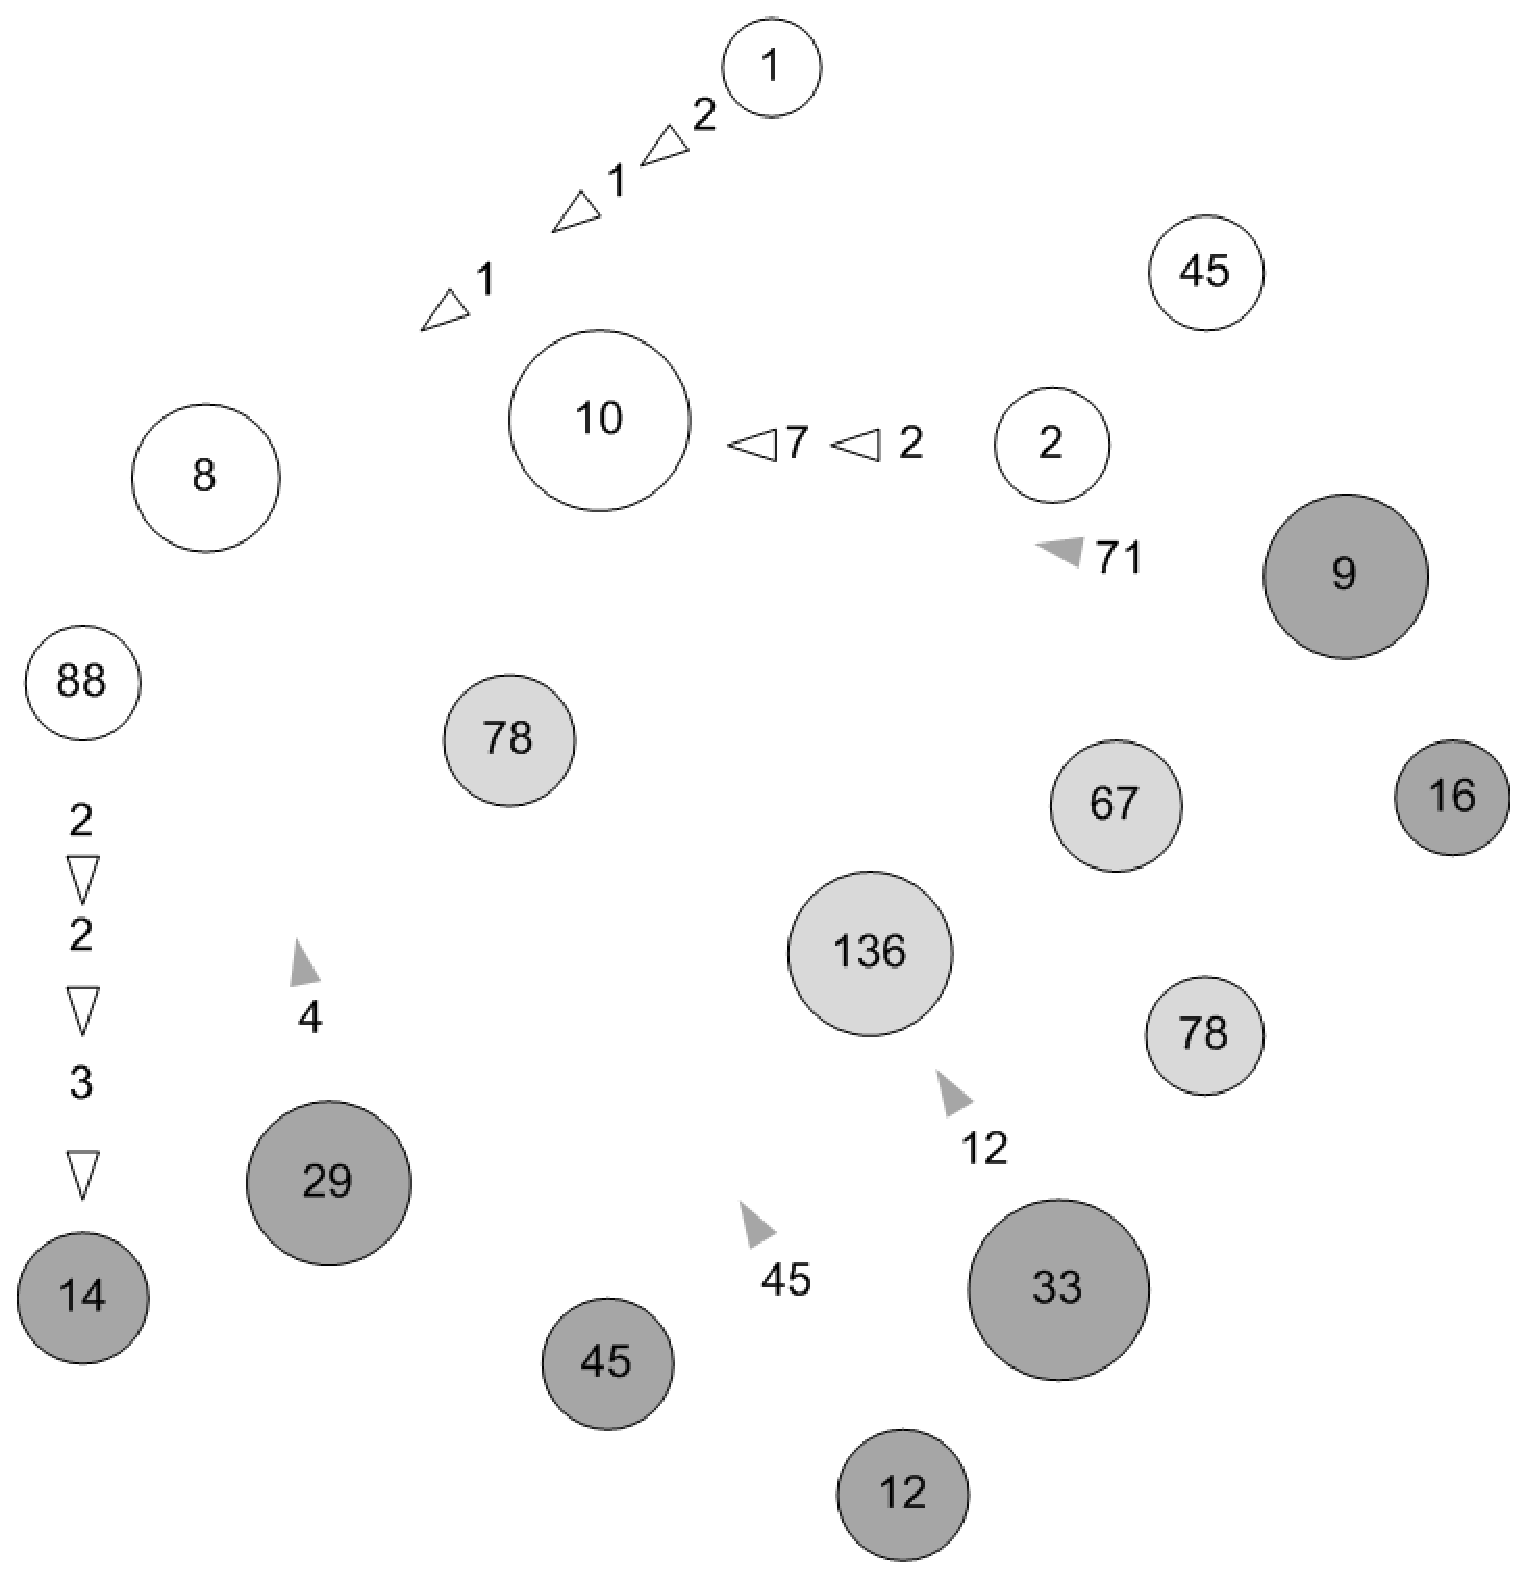
\epsfig{file=./imags/naves.eps,width=6cm}
\end{center}
\caption{Simulated screenshot of an early stage of a 1 vs 1 match in Planet Wars. White planets belong to the player (blue colour in the game), dark grey belong to the opponent (red in the game), and light grey planets belong to no player. The triangles are fleets, and the numbers (in planets and triangles) represent the ships. The planet size models the growth rate of the amount of ships in it (the bigger, the higher).}
\label{figura:PlanetWars1}
\end{figure}

A Planet Wars match takes place on a map (see Fig. \ref{figura:PlanetWars1}) that contains several planets (neutral, enemies or owned), each one of them with a number assigned to it that represents the quantity of ships that the planet is currently hosting. 

The aim of the game is to defeat all the ships in the opponent's planets. Although Planet Wars is a RTS game, this implementation has transformed it into a turn-based game, in which each player has a maximum number of turns to accomplish the objective. At the end of the match, the winner is the player that remains alive, or that who owns more ships if more than one survives. 

The problem in this paper is to create a bot's AI in order to win the game, i.e. able to defeat every possible opponent in a 1 vs 1 or 1 vs 3 match (four independent bots fighting in the same map).
The bot must react according to the state of the map in each simulated turn (input), returning a set of actions to perform in order to fight the enemy, conquering its resources, and, ultimately, wining the game. 

There are two strong constraints which determine the possible methods to apply to design a bot: a simulated turn takes \textit{just one second}, and the bot is \textit{not allowed to store any kind of information} about its former actions, about the opponent's actions or about the state of the game (i.e., the game's map).

We start from a designed bot's AI \cite{Genebot_CEC11}, named Genebot. It was defined from scratch (by an expert player), so it consists in a predefined set of behavioural rules. These rules depend on a set of parameters, which model thresholds, probabilities and weights, and which in turn, define how the bot will behave.
The set of states and parameters that the bot will consider can be seen in Figure \ref{fig:diagram}. 
%
\begin{figure*}[ht]
\begin{center}
  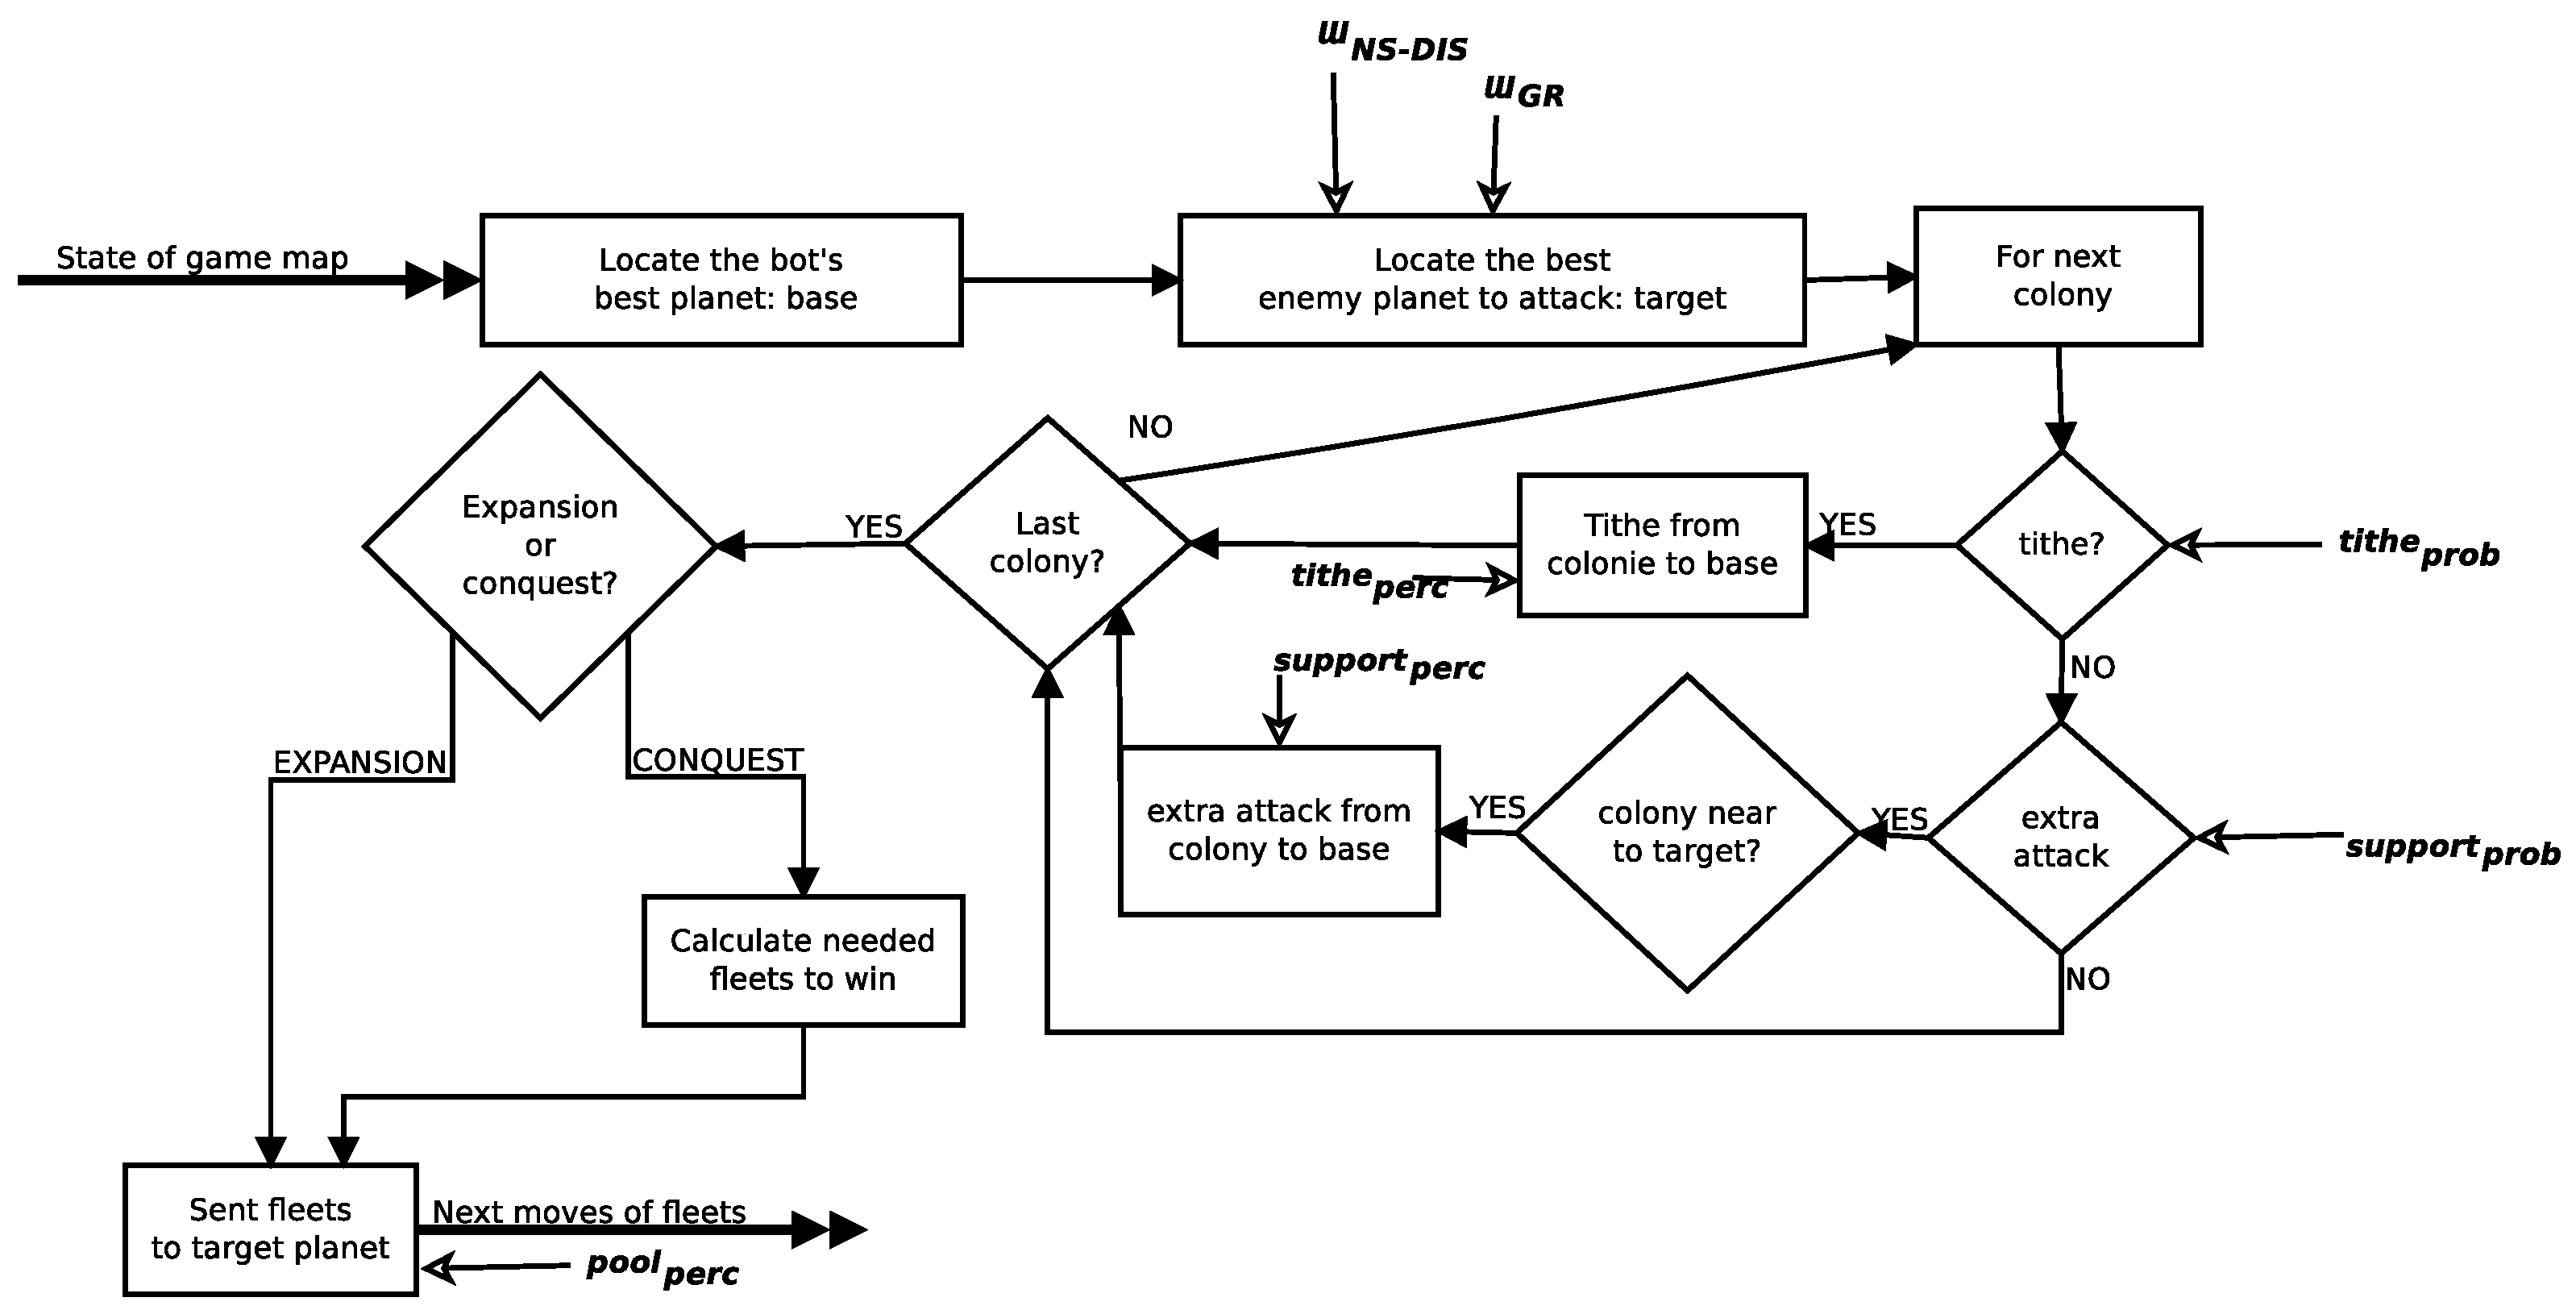
\epsfig{file=imags/diagram.eps,width=12cm}
\end{center}
\caption{Diagram of states governing the behaviour of AnonymousBot, with the parameters to be evolved highlighted. There are weights ($w$), probabilities ($prob$), and percentages ($perc$).} 
\label{fig:diagram}
\end{figure*}

Thus, the aim in this paper is to study the improvement of that set of behavioural parameters by means of some novel (in this scope) evolutionary approaches, based in the survival to evolve. These will be described in the following section.


%%%%%%%%%%%%%%%%%%%%%%%%%%%%%%%   SURVIVAL BOT  %%%%%%%%%%%%%%%%%%%%%%%%%%%%%%%%
%
\section{Survival Bots}
\label{sec:survival_bots}


% Joeves, usad comentarios!!!!

%***\\
%Contar la idea general:
%	- sustituir la evaluaci�n y el fitness
%	- selecci�n en base a supervivencia (y quiz� a antig�edad)
%	- eliminaci�n del ruido
%	- pormenores: 
%		   . 5 combates en 5 escenarios representativos
%			. rival dentro de la misma poblaci�n (auto-aprendizaje???)
%***\\

%*** tipos de codificaci�n, operadores ($BLX-\alpha$) ***

%A shape of co-evolution. They compete but the whole population (offspring) is improved.

%***All these approaches are novel, at least in the application to the present problem. The third one is completely new.***

% ------------------------------------------------------------------
%

\subsection{Bot generation using GP}
\label{subsec:generationgp}

The Genetic Programming-based bot or {\em GPBot}, presented in this work, evolves a set of rules which, in turn, models a Decision Tree. 
During the evolution, every individual in the population (a tree) must be evaluated. To do so, the tree is set as the behavioural engine of an agent, which is then placed in a map against a rival in a Planet Wars match. Depending on the obtained results, the agent (i.e. the individual) gets a fitness value, that will be considered in the evolutionary process as a measure of its validity. 
 
Thus, during the match the tree will be used (by the bot) in order to select the best strategy at every moment, i.e. for every planet a target will be selected along with the number of ships to send from one the other.

\noindent The used Decision Trees are binary trees of expressions composed by two different \textit{types of nodes}:

\begin{itemize}
\item {\em Decision}: a logical expression formed by a variable, a less than operator ($<$), and a number between 0 and 1. It is the equivalent to a ``primitive'' in the field of GP.
\item {\em Action}: a leave of the tree (therefore, a ``terminal''). Each decision is the name of the method to call from the planet that executes the tree. This method indicates to which planet send a percentage of available ships (from 0 to 1). 
\end{itemize}

\noindent The decisions are based in the values of different \textit{variables} which are computed considering some other variables in the game. They are defined by a human expert and defined in \cite{GpbotGarcia14}, and are:

\begin{itemize}
\item {\em myShipsEnemyRatio}: Ratio between the player's ships and enemy's ships.
\item {\em myShipsLandedFlyingRatio}: Ratio between the player's landed and flying ships.
\item {\em myPlanetsEnemyRatio}: Ratio between the number of player's planets and the enemy's ones.
\item {\em myPlanetsTotalRatio}: Ratio between the number of player's planet and total planets (neutrals and enemy included).
\item {\em actualMyShipsRatio}: Ratio between the number of ships in the specific planet that evaluates the tree and player's total ships.
\item {\em actualLandedFlyingRatio}: Ratio between the number of ships landed and flying from the specific planet that evaluates the tree and player's total ships.
\end{itemize}

\noindent Finally, the possible \textit{decisions} are:

\begin{itemize}
\item {\em Attack Nearest (Neutral|Enemy|NotMy) Planet}: The objective is the nearest planet.
\item {\em Attack Weakest (Neutral|Enemy|NotMy) Planet}: The objective is the planet with less ships.
\item {\em Attack Wealthiest (Neutral|Enemy|NotMy) Planet}: The objective is the planet with higher lower rate.
\item {\em Attack Beneficial (Neutral|Enemy|NotMy) Planet}: The objective is the  more beneficial planet, that is, the one with highest growth rate divided by the number of ships.
\item {\em Attack Quickest (Neutral|Enemy|NotMy) Planet}: The objective is the planet easier to be conquered: the lowest product between the distance from the planet that executes the tree and the number of  ships in the objective planet.
\item {\em Attack (Neutral|Enemy|NotMy) Base}: The objective is the planet with more ships (that is, the base).
\item {\em  Attack Random Planet}.
\item {\em Reinforce Nearest Planet}: Reinforce the nearest player's planet to the planet that executes the tree.
\item {\em Reinforce Base}: Reinforce the player's planet with higher number of ships.
\item {\em Reinforce Wealthiest Planet}: Reinforce the player's planet with higher grown rate.
\item {\em Do nothing}.

\end{itemize}

\noindent An example of a possible decision tree is shown below. This example tree has a total of 5 nodes, with 2 decisions and 3 actions, and a depth of 3 levels.

\begin{verbatim}

if(myShipsLandedFlyingRatio < 0.696)
   if(actualMyShipsRatio < 0.421)
      attackWeakestNeutralPlanet(0.481);
   else
      attackNearestEnemyPlanet(0.913);
else
   attackNearestEnemyPlanet(0.891);

\end{verbatim}\\\\

\noindent The bot's behaviour is explained in Algorithm \ref{alg:turn}.

\begin{algorithm}[ht]
\begin{algorithmic}


\STATE // At the beginning of the execution the agent receives the tree
\STATE tree $\leftarrow$ readTree()
\WHILE{game not finished}
  \STATE // starts the turn
  \STATE calculateGlobalPlanets() // e.g. Base or Enemy Base
  \STATE calculateGlobalRatios() // e.g. myPlanetsEnemyRatio
  \FOR{Each p in PlayerPlanets}
    \STATE calculateLocalPlanets(p) // e.g. NearestNeutralPlanet to p
    \STATE calculateLocalRatios(p) //e.g actualMyShipsRatio
    \STATE executeTree(p,tree)  // Send a percentage of ships to destination
   \ENDFOR
\ENDWHILE

\end{algorithmic}
\caption{Pseudocode of the proposed agent. The same tree is used during all the agent's execution}
\label{alg:turn}
\end{algorithm}

Next section will present...



\subsection{Steady-State Survival}
\label{subsec:steady-state}

This is an implementation based in the classical Steady-State EA approach \cite{Genitor_whitley}. In it, the majority of the population remains the same in the following generation, and just a small subset of individuals are substituted (usually just the worst).
This method aimed to increase the exploitation factor in the EA, since
just the worst individuals in the population are substituted by fitter
ones. % And this is interesting for this problem because... - JJ

Thus, the proposed approach follows this idea and just performs two battles per generation. The contenders are selected $RANDOMLY$ from all the population.
The best bot in 5 matches is the winner in each battle. Then, both winners are the parents for the two new individuals (offspring).
The new individuals must fight against two other random bots trying to be included in the new population.

This approach presents a higher stochastic component than the original, due to the lack of a fitness value which can value every individual with a simple number. The random selection of all the individuals increases the diversity in the algorithm run, which, in turn, could be a key factor in this problem resolution, \textcolor{red}{AS WILL BE DEMONSTRATED IN THE EXPERIMENTS}.

% ------------------------------------------------------------------
%
\subsection{Generational Survival}
\label{subsec:generational}

In this approach, as in the initial proposal \cite{GAs_Goldberg89}, half of the population is substituted every generation, having a big diversification and thus exploration factor.
In the proposed algorithm, the individuals are paired randomly,
conducting one on one battles. The winners (half of the population)
will be the parents of the next offspring. % �Y por qu� se elimina el
                                % ruido? �No puede ser que gane uno
                                % por casualidad? - JJ
Then, applying the $BLX-\alpha$ crossover, the rest of the population is generated (two descendents per couple). The parents are grouped again randomly, increasing this way the diversity/exploration of the algorithm.

% ------------------------------------------------------------------
%
\subsection{Survival Arena}
\label{subsec:arena}

This is a novel proposal in which the individuals (bots) are continuously fighting in an arena (pool).
Everyone counts with a number of life points which they lose when they are defeated in a match.

When a new individual is needed (parent), it is selected from this pool, according to its current score (\textcolor{red}{OR REMAINING LIFE POINTS}).

% ***ventajas de este m�todo***
% Pero �esto lo vais a hacer al final? NO lo mencion�is en el abstract
% - JJ


%%%%%%%%%%%%%%%%%%%%%%%%%%%%%%%   EXPERIMENTS  %%%%%%%%%%%%%%%%%%%%%%%%%%%%%%%%
%
\section{Experiments and Results}
\label{sec:experiments}

Several experiments have been conducted in order to study different issues of the proposed approaches, but having in mind that the main objective is the improvement of bots using a co-evolutionary algorithm. The set of parameters considered in the GAs is shown in Table \ref{tab:parameters}.
This set of parameters have been used previously in the work \cite{GpbotGarcia14}, obtaining competitive bots.

For each one of the presented approaches (combinations of fitness functions and knowledge-related methods), ten executions of the Co-GA have been performed.

\begin{table}
\begin{center}
\begin{tabular}{|c|c|}
\hline
{\em Parameter Name} & {\em Value} \\\hline \hline
Population size & 32 \\\hline
Crossover type & Sub-tree crossover \\ \hline
Crossover rate & 0.5\\ \hline
Mutation  & 1-node mutation\\ \hline
Mutation step-size & 0.25 \\ \hline
Selection & 2-tournament \\ \hline
Replacement & Steady-state\\ \hline
Stop criterion & 50 generations \\ \hline
Maximum Tree Depth & 7  \\ \hline 
Runs per configuration & 30 \\ \hline 
Maps used in each evaluation & map76, map69, map7, map11, map26 
\\ \hline
\end{tabular}
\caption{Parameters used in the experiments.}
\label{tab:parameters}
\end{center}
\end{table}

%%%%%%%%%%%%%%%%%%%%%%%%%%%%%%  CONCLUSIONS  %%%%%%%%%%%%%%%%%%%%%%%%%%%%%%%
%
\section{Conclusions and Future Work}
\label{sec:conclusions}

This paper presents four different implementations of a quite simple approach: to omit the fitness-based selection mechanism in an EA. 

This has been applied over the improvement of the behavioural parameters of the bot's AI in the RTS game Planet Wars. Then, the tournament has been modelled as a battle in the game



The results obtained in this study are very promising, but they inherit a flaw from previous works, which is the low flexibility level due to the predefined set of rules/states that the bots follow. This means that almost every bot will eventually behave well, and the diversity in the search loses its relevance.
The consideration of a more flexible approach for defining the behavioural engine of the bots, such as a Genetic Programming one [REF GP Genebot], could yield more interesting results and conclusions about the value of the methods proposed in this work.

%ACKNOWLEDGMENTS are optional
\section{Acknowledgments}
This paper has been funded in part by European and National projects FP7-318508 (MUSES) and TIN2011-28627-C04-02 (ANYSELF) respectively, project P08-TIC-03903 (EV\-ORQ) awarded by the Andalusian Regional Government, and project 83 (CANUBE) awarded by the CEI-BioTIC UGR.

\bibliographystyle{IEEEtran}
\bibliography{genebot}

\end{document}
